
An example of a figure is is \autoref{fig:trends}. And also \autoref{tab:exampletable}. They can be referenced by using \texttt{autoref} or \texttt{ref}.\todo{There is also todos that can be useful} You can also reference chapters like this: "You can read about my results in chapter \ref{ch:results}". Citations are defined in \texttt{references.bib}, and here is an example\cite{eghbal2020working}.

\begin{figure}
	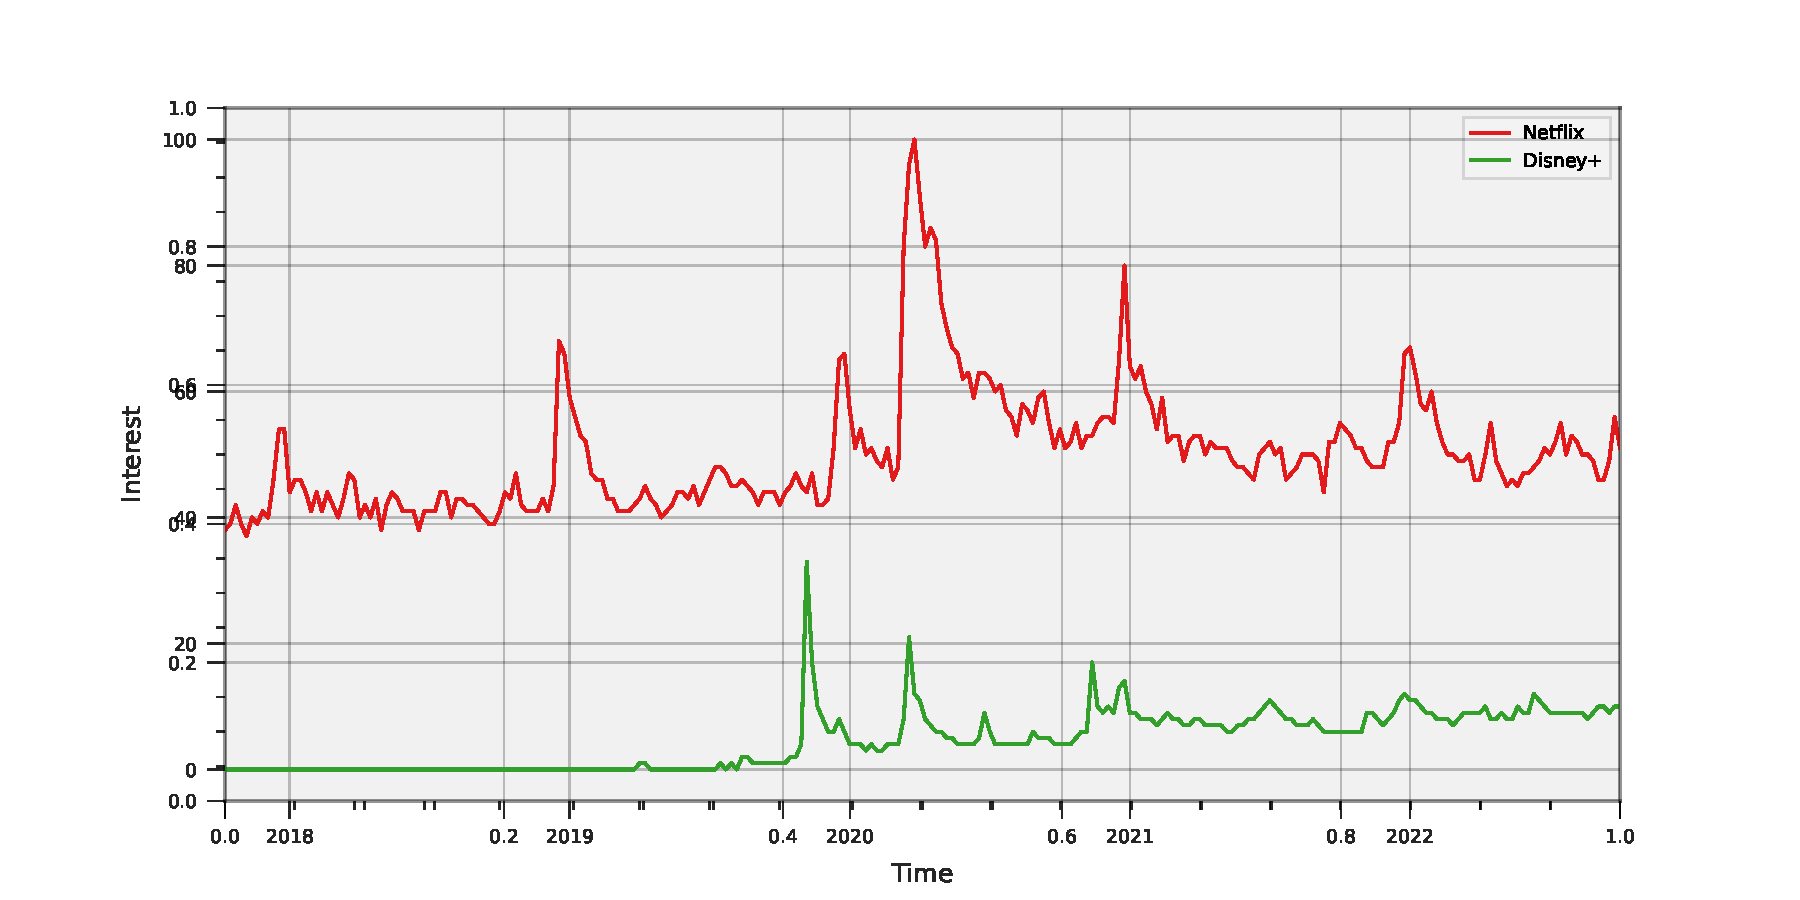
\includegraphics[width=\linewidth]{assets/trends.pdf}
	\caption{Google Trends data showing interest over time of Netflix and Disney+}\label{fig:trends}
\end{figure}

\begin{table}[ht]
	\centering
	\begin{tabular}{lll}
		\bf{Email provider} & \bf{Unique email addresses} & \bf{Commit count} \\
		gmail.com       & 1279  & 9091  \\
		google.com      & 661   & 56355 \\
		github.com      & 476   & 2622  \\
		intel.com       & 76    & 1918  \\
	\end{tabular}
	\caption{The most common email addresses for commits to TensorFlow}\label{tab:exampletable}
\end{table}
